\documentclass{beamer}
\usepackage[pangram]{blindtext}
%\usetheme{Pittsburgh}
\usepackage[utf8]{inputenc}
\usepackage[T1]{fontenc}
\usepackage{graphicx}
\usepackage{tikz}
\usetikzlibrary{positioning, fit}
\usetikzlibrary{calc, angles, intersections, quotes, through}
\usepackage{amsmath}
\usepackage{amssymb}
\usepackage{siunitx}
\usepackage{multirow}
\usepackage{makecell}
\usepackage{longtable}
\setbeamertemplate{caption}[numbered]
%\usepackage{subcaption}
\usepackage{tikz}
\usepackage{listings}
\usetikzlibrary{calc}
\usepackage{listings}
\usepackage{subfig}
\usepackage{ifthen}
\tikzset{point/.style={circle, inner sep=0pt, minimum size=3pt, fill=red}}
\usetikzlibrary{shapes}
\newlength{\pvlength}
\def\RTUpresdef{\string~/RTUpresdef}

\title{Studies of colour flow in top quark pair decays at 13 TeV}
\subtitle{Results at the CMS experiment of the CERN LHC\\\vspace{0.5cm}CMS AN-17-309}
\author{Viesturs Veckalns}
\institute{Rīgas Tehniskā universitāte}
\date{Top Event Modelling and Generators - Physics Meeting, ****, 2019}


\usepackage{xparse,calc}
%\logo{\raisebox{-6cm}{\includegraphics[width=1cm]{CMS_logo_May2014-eps-converted-to.pdf}}}

%\makeatletter
\input{\RTUpresdef/presdefinitions.tex}
\newcommand{\DeltaR}{\ensuremath{\Delta R^{}}\xspace}
\newcommand{\leadingjet}{\ensuremath{j_{1}^{W}}\xspace}%
\newcommand{\scndleadingjet}{\ensuremath{j_{2}^{W}}\xspace}%
\newcommand{\leadingb}{\ensuremath{j_{1}^{b}}\xspace}%
\newcommand{\scndleadingb}{\ensuremath{j_{2}^{b}}\xspace}%
\newcommand{\hadronicb}{\ensuremath{j_{\text{h}}^{b}}\xspace}%
\newcommand{\pullangle}{\ensuremath{\theta_{\text{p}}}\xspace}%
\newcommand{\pullvector}{\ensuremath{\vec{P}}\xspace}%
\newcommand{\pvmag}{\ensuremath{\left|\vec{P}\right|}\xspace}%
\newcommand{\pval}{$p$-value}%

\newcommand{\jettitle}[1]{%
\ifthenelse{\equal{#1}{leading_jet}}{\leadingjet}{}%
\ifthenelse{\equal{#1}{scnd_leading_jet}}{\scndleadingjet}{}%
\ifthenelse{\equal{#1}{leading_b}}{\leadingb}{}%
\ifthenelse{\equal{#1}{scnd_leading_b}}{\scndleadingb}{}%
}%

\newcommand{\countertitle}[1]{%
\ifthenelse{\equal{#1}{leading_jet}}{\scndleadingjet}{}%
\ifthenelse{\equal{#1}{scnd_leading_jet}}{\leadingjet}{}%
\ifthenelse{\equal{#1}{leading_b}}{\scndleadingb}{}%
\ifthenelse{\equal{#1}{scnd_leading_b}}{\leadingb}{}%
}%


\newcommand{\observabletitle}[1]{%
\ifthenelse{\equal{#1}{pull_angle}}{pull angle \pullangle}{}%
\ifthenelse{\equal{#1}{pvmag}}{magnitude of the pull vector \pvmag}{}%
}%

\newcommand{\chargetitle}[1]{%
\ifthenelse{\equal{#1}{allconst}}{all jet constituents}{}%
\ifthenelse{\equal{#1}{chconst}}{only charged jet constituents}{}%
}%

\newcommand{\methodtitle}[1]{%
\ifthenelse{\equal{#1}{nominal}}{\ensuremath{t\overline{t}}\xspace}{}%
\ifthenelse{\equal{#1}{cflip}}{\ensuremath{t\overline{t}\ \text{cflip}}\xspace}{}%
}%

\newcommand{\binningtitle}[1]{% 
  \ifthenelse{\equal{#1}{ORIG}}
             {the original binnning}
             {}%    
  \ifthenelse{\equal{#1}{ATLAS3}}{3 regularly sized bins}{}%
  \ifthenelse{\equal{#1}{SIGMA_0p1}}{the optimised binning with a $\sigma$ factor of 0.1}{}%
  \ifthenelse{\equal{#1}{SIGMA_0p6}}{the optimised binning with a $\sigma$ factor of 0.6}{}%
}%           

\newcommand{\flowtitle}[1]{%
\ifthenelse{\equal{#1}{N}}{particle}{}%
\ifthenelse{\equal{#1}{E}}{energy}{}%
\ifthenelse{\equal{#1}{Pt}}{\ensuremath{p_{T}}\xspace}{}%
}%

\newcommand{\recoleveltitle}[1]{%
\ifthenelse{\equal{#1}{gen}}{generator}{}%
\ifthenelse{\equal{#1}{reco}}{reconstruction}{}%
}%

\newcommand{\modeltitle}[1]{%
\ifthenelse{\equal{#1}{nominal}}{SM}{}%
\ifthenelse{\equal{#1}{cflip}}{colour octet $W$}{}%
}%

\def\customwidth{\textwidth}

%% \ExplSyntaxOn
%% \NewExpandableDocumentCommand{\capitalise}{m}{\tl_mixed_case:n{#1}}
%% \ExplSyntaxOff

\usepackage{xspace}
\usepackage{ptdr-definitions}

\begin{document}
{
  \usebackgroundtemplate{\includegraphics[width=\paperwidth]{\RTUpresdef/pamats1.jpg}}%
  \setbeamertemplate{footline}{}
  \logo{}
  \begin{frame}
    \fitimage{%
      \titlepage
      %\blindenumerate[2]
    }{example-image-a}
  \end{frame}
}

\begin{frame}{Collaborators}
  \begin{itemize}
    \item Martijn Mulders (CERN)
    \item Pedro Silva (CERN)
    \item Markus Seidel (CERN)
  \end{itemize}
\end{frame}

\begin{frame}{Colour flow in \ttbar decays}
  \centering
    \includegraphics[width = 0.9\paperwidth]{presfig/ttbar_cf_labels_en.pdf}
\end{frame}

\section{Methodology}
\section{Pull angle}

An explanation about the coordinate system used at CMS is in order. The CMS uses coordinate system centred on the nominal collision point, the $x$ points towards the centre of the LHC, the $y$ axis points upwards and the $z$ axis points along the beam in the direction of the Jura mountains - see Fig. \ref{fig:CMScoordinates}. $\rho$ is the radial coordinate. The azimuthal angle $\phi$ is measured from the $x$ axis to the projection of the spatial vector $\textbf{p}$ in the $x-y$ plane. The polar angle $\theta$ is measure from the positive direction of the beam to the vector $\textbf{p}$. Pseudorapidity $\eta$ is defined as

\begin{equation}
\eta\equiv-\ln\left(\frac{\theta}{2}\right).
\end{equation}

The pseudorapidity is equal to

\begin{equation}
\eta=\ln\left(\frac{p+p_{L}}{p-p_{L}}\right),
\end{equation}

where $p$ is the magnitude of $\textbf{p}$ and $p_{L}$ is the longitudinal component of $\textbf{p}$ along the direction of the beam.
A measurement related to pseudorapidity is the rapidity $y$ defined as:

\begin{equation}
y\equiv\ln\left(\frac{E+p_{L}}{E-p_{L}}\right),
\end{equation}

where $E$ is the energy of the particle. For massless particles rapidity and pseudorapidity are equal. For our present purposes, rapidity and pseudorapidity can be used interchangeably without a loss of accuracy.

\begin{figure}[hptb]
  \centering
  \includegraphics[width=0.7\textwidth]{fig/coordinates/coordinates.pdf}
  \caption{The coordinate system of CMS.}
  \label{fig:CMScoordinates}
\end{figure}

We adopt the methodology proposed by \cite{Gallicchio:2010sw} to use the pull angle to reveal colour connection between two quark jets. The pull angle $\theta_{p}$ formed by the pull vector $\vec{v}_{p}$ and difference between two jets $\vec{J}_{2}-\vec{J}_{1}$ is shown in Fig. \ref{fig:pull_angle}. The $\phi$-$y$ coordinate system is used. 

\begin{figure}[hbtp]
  \centering
  \includegraphics[width=1.0\textwidth]{fig/pull_angle.pdf}
  \caption{Pull angle $\theta_{p}$, pull vector $\vec{v}_{p}$ in a $y$-$\phi$ plane.}
  \label{fig:pull_angle}
\end{figure}

The pull vector is given by the formula

\begin{equation}
  \vec{v}_{p}=\sum_{i\in J}\frac{p^{T}_{i}|\vec{r}_{i}|}{p^{T}_{J}}\vec{r}_{i},
  \label{Eq:pull_angle}
\end{equation}

where $i$ is the index of the constituent of jet $J$, $p^{T}_{i}$ is the transverse moment of the jet constituent, $\vec{r}_{i}$ is the vectorial difference between the jet component and the jet, $p^{T}_{J}$ - the transverse moment of the jet.

Two jets that are colour connected are expected to have jet constituents dispersed in the area between the two jets. Hence the pull vector of $J_{1}$ would point towards $J_{2}$ and the pull angle would be narrow. For jets that are not colour connected the pull angle is expected to be distributed isotropically.

The methodology of the pull angle has been applied in the \DZERO experiment of Tevatron \cite{Abazov:2011vh} and the ATLAS experiment at the LHC in Run I \cite{Aad:2015lxa} and in Run II \cite{ATLAS:2017iaz}. We hope to outperform all results with the methodology of the pull angle with the state-of-the-art tracker of the CMS detector immersed in the 4 T magnetic field of the superconducting solenoid.

The anti-$k_{T}$ clustering algorithm ensures a conical jet shape in case the jet separation \DeltaR is more than double of the parameter $R$, which is set at 0.4 at CMS. This case is illustrated in Fig. \ref{fig:anti_kt_a}. In case of separation between jets \DeltaR being less than double of the parameter $R$ the hard jet will wean constituents from the soft jet. This is illustrated in Fig. \ref{fig:anti_kt_b}. This latter effect will have consequences for the colour flow analysis with the pull angle as it will induce a pull from the involved jets to each other. This warrants a separation of the cases $\DeltaR\leq2R$, $\DeltaR>2R$. 

\begin{figure}[hbtp]
  \def\twidth{0.5}
  \subfloat[$\Delta_{ij}=3.15$.]{
    \includegraphics[width=\twidth\textwidth]{fig/dR-3p150-pt2-075.pdf}
    \label{fig:anti_kt_a}
  }%
 \subfloat[$\Delta_{ij}=1.95$.]{
    \includegraphics[width=\twidth\textwidth]{fig/dR-1p950-pt2-075.pdf}
    \label{fig:anti_kt_b}
  }
   \caption{Jet shapes obtained with the anti-$k_{t}$ clustering. $R=1.5$ is used. Two cases are shown - $\Delta_{ij}=3.15$ and  $\Delta_{ij}=1.95$. The \pt of the hard jet is 100 GeV, the \pt of the soft jet is 75 GeV. Courtesy of Cacciari, Salam and Soyez.}
  \label{fig:anti_kt}
\end{figure}

Tracking efficiency of the detector is not perfect. It depends on the quality of the track finder algorithm and properties of the detector such as geometrical acceptance and material content. Fig. \ref{fig:2011_trackPerformance_MC_SingleParticles_pi_efficiencyVsPt}  shows the tracking efficiency of pions, a particle commonly resulting from quark hadronisation. Tracking efficiency is defined as the fraction of simulated charged particles that can be associated with corresponding reconstructed tracks. The tracking efficiency drops at low \pt of the particle. In our analysis we choose 1.0 GeV as the threshold and exclude particles whose \pt is below it from our analysis.

\begin{figure}[hbtp]
    \includegraphics[width=0.6\textwidth]{fig/figs_2011_trackPerformance_MC_SingleParticles_pi_efficiencyVsPt.png}
    \caption{Track reconstruction efficiencies for pions passing the high-purity quality requirements. Results are shown as a function of \pt (right), for the barrel, transition, and endcap regions, which are defined by the $\eta$ intervals of 0 - 0.9, 0.9 - 1.4 and 1.4 - 2.5, respectively. \cite{Chatrchyan:2014fea}}
    \label{fig:2011_trackPerformance_MC_SingleParticles_pi_efficiencyVsPt}
\end{figure}

\section{LEP method}

Another methodology of studying colour-connected jets in the process $e^{+}e^{-}\rightarrow q\overline{q}q\overline{q}$ at \sqrts=189-207 \GeV was used in various experiments of LEP (\cite{Abdallah:2006uq}, \cite{Abbiendi:2005es}, \cite{Achard:2003pe}). Two inter-\PW planes formed by colour-connected quarks and two intra-\PW planes formed by quarks that are not colour connected are introduced as shown in Fig. \ref{fig:LEP_method}. Particles are projected onto these planes and the angle with the leftmost quark $\chi_{1}$ is taken. If this angle is less than the angle $\chi_{0}$ between the quarks forming the plane (which means the particle is projected between the respective quarks) then the normalised angle $\chi_{R}=\frac{\chi_{1}}{\chi_{0}}$ is plotted in the region corresponding to the plane after a linear transformation

\begin{equation}
  \chi=\chi_{R} + n_{\text{plane}} - 1
\end{equation}

has been performed on the normalised angle. 

\begin{figure}[hbtp]
  \centering
  \includegraphics[width=0.6\textwidth]{fig/L3method.pdf}
  \caption{Inter-\PW and intra-\PW planes in the process $e^{+}e{-}\rightarrow q\overline{q}q\overline{q}$ and the relative angle $\chi_{R}=\frac{\chi_{1}}{\chi_{0}}$.}
  \label{fig:LEP_method}
\end{figure}

In the \ttbar semileptonic decay an arrangament as shown in Fig. \ref{fig:LEP_method} is not possible. Therefore a modification as shown in Fig. \ref{fig:LEP_method_adaptation} is proposed. There is one plane formed by colour connected jets - the leading light jet \leadingjet and the second leading light jet \scndleadingjet from the hadronic decay of the \PW boson. Additionally there are 3 colour-free regions formed by 1) the furthest light jet $j^{W}_{f}$ and the hadronic \cPqb jet \hadronicb 2) the hadronic \cPqb jet \hadronicb and the closest light jet $j^{W}_{c}$, 3) the leading \cPqb jet \leadingb and the second leading \cPqb jet \scndleadingb. Whether a jet is close or far is determined with regard to the angle between jets in the Euclidian space. In the regions shown in Fig. \ref{fig:LEP_method_adaptation_qfhb} and Fig. \ref{fig:LEP_method_adaptation_hbqc} we may hope to observe colour reconnection effects.

\begin{figure}[hbtp]
  \centering
  \def\twidth{0.24}
  \subfloat[Colour-connected region \leadingjet - \scndleadingjet.]{%
    \includegraphics[width=\twidth\textwidth]{fig/LEP_adaptation/qlq2l.pdf}%
    \label{fig:LEP_method_adaptation_qlq2l}
  }\hfil
 \subfloat[Colour-free region $j^{W}_{f}$ - \hadronicb.]{%
    \includegraphics[width=\twidth\textwidth]{fig/LEP_adaptation/qfhb.pdf}%
    \label{fig:LEP_method_adaptation_qfhb}
 }\hfil
  \subfloat[Colour-free region \hadronicb - $j^{W}_{c}$.]{%
    \includegraphics[width=\twidth\textwidth]{fig/LEP_adaptation/hbqc.pdf}%
    \label{fig:LEP_method_adaptation_hbqc}
  }\hfil
  \subfloat[Colour-free region \leadingb - \scndleadingb.]{%
    \includegraphics[width=\twidth\textwidth]{fig/LEP_adaptation/blb2l.pdf}%
    \label{fig:LEP_method_adaptation_blb2l}
  }
  \caption{Adaptation of the LEP method to \ttbar semileptonic decay involving a colour - connected region and 3 colour-free regions.}
  \label{fig:LEP_method_adaptation}
\end{figure}

The method calls for a separation of hadronic and leptonic \cPqb quarks. Each \cPqb quark is paired to each \PW boson and the invariant mass is compared to the mass of the \cPqt quark - 173.34 \GeV. The \cPqb quark is assigned to the branch where the difference of the masses is the smallest. 


\begin{frame}{Colour octet \PW boson}
  \centering
  \includegraphics[width=0.7\textwidth]{fig/ttbar_cf_flip_cropped.pdf}
\end{frame}

\section{Event Selection}
The goal of event selection is to separate signal from background. Separate selection is applied to detector level MC events and generator level MC events. Simulated events are tagged as passing only the reconstruction-based, only the particle-based or both selections. The selection for data is that of the detector level MC events.

The discussion of this section is adapted from~\cite{CMS-AN-2017-159}, which uses a similar event selection.

\section{Detector level}
\label{sec:detector_level}

The event selection is based on the \ttbar$\to$lepton+jets decay topology where one of the \PW bosons decays to a charged lepton ($\ell=e, \mu$) and a corresponding neutrino, while the other \PW boson decays to quarks yielding jets.

The particle flow PF algorithm is used for reconstruction of final state objects~\cite{Sirunyan:2017ulk}. This algorithm combines signals from all sub-detectors to enhance the reconstruction performance and it allows to identify muons, electrons, photons, charged hadrons and neutral hadrons produced after a \Pp\Pp collision.

Data samples are collected using the single lepton trigger paths of the High Level Trigger summarised in Table~\ref{tab:triggers}.

\begin{table}[htp]
\centering
\caption{Trigger paths used for online selection in the analysis.}
\label{tab:triggers}
\begin{tabularx}{\linewidth}{lllXX}\hline
Final state                 & Path                                & Run range & Function & L1 seed\\\hline
e+jets                      & \small HLT\_Ele32\_eta2p1\_WPTight\_Gsf\_v & all       & \small Select $e$ with $\left|\eta\right|<2.1$ and $\pt>32$ with the tight working point and using the GSF to reconstruct tracks
                                                                                         & \small L1\_SingleEG40\newline OR\newline L1\_SingleIsoEG22er\newline OR\newline L1\_SingleIsoEG24er\newline OR\newline L1\_SingleIsoEG24\newline OR\newline L1\_SingleIsoEG26\\\hline
\multirow[t]{2}{*}{$\mu$+jets}
                            & \small HLT\_IsoMu24\_v                     & all       & \small Select isolated $\mu$ with $\pt>20$~\GeV using L3 tracker algorithm
                                                                                         & \multirow[t]{2}{*}{\small L1\_SingleMu18}\\
                            & \small HLT\_IsoTkMu24\_v                   & all       & \small Select isolated $\mu$ with $\pt>20$~\GeV using HLT tracker muon algorithm
                            & \\\hline
\end{tabularx}
\end{table}

Offline, we require exactly one tight electron/muon with $\pt>34/26\GeV$ and $|\eta|<2.1/2.4$. The tight working point allows to identify an electron/muon when it is really an electron/muon, important in a high background environment.
The event is vetoed in the presence of a second loose lepton with $\pt>15\GeV$ and $|\eta|<2.4$.

The events are required to have in addition four jets clustered with the anti-$k_{T}$ algorithm with jet separation $R=0.4$ and charged hadron subtraction (we use shorthand AK4PFchs) with $\pt>30\GeV$  and $|\eta|<2.4$. The motivation for selecting high \pt physics objects is that the detector efficiency drops at low \pt.

At least two jets are required to be \cPqb-tagged by the Combined Secondary Vertex algorithm (CSVv2) medium working point. 

At least two untagged (light) jets are required to yield a \PW boson candidate with an invariant mass $\left|m_{jj}-80.4\right|<15~\GeV$.

The event yields at different selection stages are shown in Fig.~\ref{fig:_reco_selection} and Table~\ref{tab:yields}. Table~\ref{tab:yields_cflip} shows the event yields for the colour octet \PW sample. The estimated signal fraction of the signal increases from 0.1~\%in the initial selection stage to 94.2~\% at the final selection stage - this is a measure of efficiency of our selection.

\figureEML{/reco/}{_reco_selection}{Event yields at different stages of selection: $1 \ell$, $1 \ell+\geq 4j$, $1 \ell+\geq 4j (2b)$, $1 \ell+\geq 4j (2b, 2lj)$.}

\input{tables/event_yields_tables/event_yields_table.txt}

\input{tables/event_yields_tables/event_yields_table_cflip.txt}


\section{Generator level}
\label{sec:generator_level}

In the simulation, the offline selection is mimicked at particle level using the \PSEUDOTOPPRODUCER tool~\cite{code:pseudotop}, using a common lepton selection for both electrons and muons of $\pt>26\GeV$ and $|\eta|<2.4$, and otherwise jet $\pt/\eta$ ($\pt>30~\GeV$, $|\eta|<2.4$) and W mass requirements ($\left|m_{jj}-80.4\right|<15~\GeV$) identical to the offline selection.

Charged leptons stemming from the hard process are dressed with nearby photons in a $R=0.1$ cone, and jets are clustered with the anti-$k_T$ algorithm with  $R=0.4$ cone after removing the dressed leptons as well as all neutrinos. In order to identify the flavour of the jet at particle level, ``ghost'' B-hadrons are included in the clustering after scaling their momentum by $10^{-20}$ in order that they do not change significantly the jet energy scale at particle level.


\section{Corrections and systematics}
\input{presxxx/systematics.tex}

\section{Results}
\label{chap:results}
\section{Notikumu attēls}
\ref{fig:event_display}. att. redzams notikums, kuru veido vieglās strūklas, \cPqb kvarku strūklas un leptons $\eta-\phi$ plaknē. Attēlots arī vilkmes vektors. Attēls veidots līdzīgi kā \ref{fig:pull_angle}. att.

\begin{figure}[hbtp]
  \centering
  \includegraphics[width=1.0\textwidth]{fig/individual_plots/reco_allconst_total_1111_DeltaR_2p846131_pull_angle_1p964620.png}
  \caption{Vadošās strūklas vilmes vektors (pārtraukta līnija ar punktiem), kas veido 1.96 rad vilkmes leņķi ar vektoriālo starpību (pārtraukta līnija) starp otro vadošo vieglo strūklu un vadošo vieglo strūklu. Vadošās strūklas sastāvdaļas ir attēlotas ziā, krāsā, bet otrās vadošās strūklas sastāvdaļas ir attēlotas sarkanā krāsā. Vadošā strūkla ir attēlota ar nepārtrauktau līniju, bet otrā vadošā strūkla ir attēlota ar pārtrauktu līniju. Hadroniskā \cPqb kvarka strūkla un tās sastāvdaļas attēlotas zaļā krāsā, bet leptoniskā \cPqb kvarka strūkla un tās sastāvdaļas attēlotas violetā krāsā. Vilkmes vektors ir palielināts 200 reizes, bet apļiem, kas attēlo strūklas, radiuss ir vienās ar $\frac{p_{T}}{75.0}$, savukārta apļiem, kas attēlo strūklu sastāvdaļas, radiuss ir vienās ar $\frac{p^{\text{constituent}}_{T}}{p^{\text{jet}}_{T}}$.}
  \label{fig:event_display}
\end{figure}

\section{Vilkmes vektors}

Pētījuma veikšanai tika izstrādāts rīku kopums \textsc{CFAT} \cite{url:cfat}. Galvenā pētījumu daļā tika veikta, izmantojot \CMSSW versiju \lstinline[language=sh]|CMSSW_8_0_26_patch1|. Grafiki ir veidoti, izmantojot \ROOT \cite{Brun}. Vilkmes vektori tiek noteikti visāmm novērojamajām strūklā - vadošajai vieglajai strūklai \leadingjet (ar vislielāko \pt), otrajai vadošajai vieglajai strūklai \scndleadingjet, vadošajai hadroniskā \cPqb strūklai \leadingb un otrajai vadošajai hadroniskā \cPqb strūklai \scndleadingb. Visos gadījumos, tiek izdalīti apakšgadījumus, iekļaujot vilkmes vektora aprēķinā visas strūklaas sastāvdaļās vai tikai elektriski lādētās sastāvdaļas. Rezultāti ir izdalīti pa $e$ + strūklas0, $\mu$ + strūklas un kopējo leptons + strūklas kanāliem.

$\eta$ dimensija vilkmes vektoram ar visām strūklas sastāvdaļām ir attēlots \ref{fig:_eta_PV_allconst_reco_leading_jet}. - \ref{fig:_eta_PV_allconst_reco_leading_jet}. att.

Vietā ir paskaidrojums par KMS grafiku formātu. Augšējais grafiks \ref{fig:_eta_PV_allconst_reco_leading_jet}. att. attēlo datus un Monte Karlo simulācijas. Ja nav norādīts citādi, Monte Karlo simulācijas ir attēlotas rekonstrukcijas līmenī. Zilā josla attēlo sistemātiskās nenoteiktības. Ja dota sistemātskā nenoteiktība ar indeksu $k$ mēs to identificējam kā pozitīvu sistemātiku $U^{k}_{i}$, ja vērtības intervālā $i$ sistemātika $S^{k}_i$ pārsniedz nominālo vērtību $N_{i}$. Pretējā gadījuma sistemātiskā nenoteiktība tiek noteikta kā negatīva sistemātikā nenoteiktība $D^{k}_{i}$. Kopējā pozitīvā un negatīvā sistemātiskā nenoteiktība tiek noteikta kā kvadrātu summa:

\begin{align}
U_{i}=\sqrt{\sum_{k}\left(U^{k}_{i}-N_{i}\right)^{2}} && D_{i}=\sqrt{\left(\sum_{k}D^{k}_{i}-N_{i}\right)^{2}}.
\end{align}

Zilās joslas platums atbilst sistemātiskajai kļūdai, kas noteikta kā $\frac{U_{i}+D_{i}}{2}$. Joslas centrs atbilst $N_{i} + \frac{U_{i}-D_{i}}{2}$. Teiktais attiecas arī uz rozā joslu ar atšķirību, ka sistemātikas ir tikušas normalizētas ar signāla integrāli (šādas normalizētas histogramas tiek sauktas par \gls{veidoliem}). Apakšejā ielikumā attēlota datu attiecība pret Monte Karlo, kā arī sistemātikas, kas normalizētas pret Monte Karlo.

\figureEML{/reco/PV/charge/allconst/}
          {_eta_PV_allconst_reco_leading_jet}
          {\leadingjet vilkmes vektora $\eta$ dimensija, iekļaujot visas strūklas sastāvdaļas.}

\leadingjet vilkmes vektora  $\phi$ dimensija, ieļaujot visas strūklas sastāvdaļas ir attēlota \ref{fig:_phi_PV_allconst_reco_leading_jet}. - \ref{fig:_phi_PV_allconst_reco_leading_jet}. att. 

\figureEML{/reco/PV/charge/allconst/}
          {_phi_PV_allconst_reco_leading_jet}
          {\leadingjet vilkmes vektora $\phi$ dimensija, iekļaujot visas strūklas sastāvdaļas.}

Vilkmes vektora lielums ar visām strūklu komponentēm ir attēlots \ref{fig:_mag_PV_allconst_reco_leading_jet} - \ref{fig:_mag_PV_allconst_reco_leading_jet}. att. Vilkmes vektora lielums parasti nepārsniedz 0.02 [bez mērvienības].

\figureEML{/reco/PV/charge/allconst/}
          {_mag_PV_allconst_reco_leading_jet}
          {\leadingjet vilkmes vektora lielums, iekļaujot visas strūklas sastāvdaļas.}

\section{Vilkmes leņķis}

Vilkmes leņķa distribūcija starp ar krāsām saistītām strūklām - no \leadingjet uz \scndleadingjet ar visām strūklu komponentēm un ar jebkuru \DeltaR ir attēlota \ref{fig:_pull_angle_allconst_reco_leading_jet_scnd_leading_jet_DeltaRTotal}. att.

\figureEML{/reco/pull_angle/DeltaRTotal/charge/allconst/}
          {_pull_angle_allconst_reco_leading_jet_scnd_leading_jet_DeltaRTotal}
          {Vilkmes leņķā distribūčija no \leadingjet uz \scndleadingjet ar jebkuru \DeltaR un iekļaujot visas strūklu komponentes.}


\ref{fig:_pull_angle_allconst_reco_leading_b_scnd_leading_b_DeltaRTotal}. att. attēlotas vilkmes leņķa distribūcijas, gadījumos, kas nav sagaidāma krāsu saistība starp strūklām - no \leadingb uz \scndleadingb un no \scndleadingb uz \leadingb iekļaujot visas strūklu sastāvdaļās un pie visām \DeltaR vērtībām.

\figureEML{/reco/pull_angle/DeltaRTotal/charge/allconst/}
          {_pull_angle_allconst_reco_leading_b_scnd_leading_b_DeltaRTotal}
          {Vilkmes leņķa no \leadingb uz \scndleadingb distribūcija pie visām \DeltaR vērtībām un iekļaujot visas strūklu sastāvdaļas.}

Papildu iespēja novērto vilkmes leņķa distribūciju starp objektiem, starp kuriem nav krāsu saistība, ir izvēlēties strūklu un leptonu. \ref{fig:_pull_angle_allconst_reco_leading_jet_lepton_DeltaRTotal}. att. attēlota vilkmes leņķā distribūcija starp \leadingjet un lādēto leptonu. 

\figureEML{/reco/pull_angle/DeltaRTotal/charge/allconst/}
          {_pull_angle_allconst_reco_leading_jet_lepton_DeltaRTotal}
          {Vilkmes leņķa distribūcija no \leadingjet uz lādēto leptonu pie visām \DeltaR vērtībām un iekļaujot visas strūklu sastāvdaļas.}

Attēlos redzams, ka centrālais paugurs vilkmes leņķa distribūcijā ir acīmredzams, ja iesaistītas ar krāsām saistības strūklas, kā arī tas izlīdzinās, ja ir iesaistīti ar krāsām nesaistīti objekti. 

Centrālais paugurs var būt redzams gadījumos, ja starp fizikālo objektu vekotriem pastāv kolinearitāte, kaut arī paši fizikas objekti nav saistīti ar krāsām. Šāds gadījums redzams, apskatot vilkmes leņķa distribūciju no \leadingjet uz hadronisko \PW - \ref{fig:_pull_angle_allconst_reco_leading_jet_had_w_DeltaRTotal}. att. 

\figureEML{/reco/pull_angle/DeltaRTotal/charge/allconst/}
          {_pull_angle_allconst_reco_leading_jet_had_w_DeltaRTotal}
          {Vilkmes leņķa distribūcija no \leadingjet uz hadronisko \PW pie visām \DeltaR vērtībām un iekļaujot visas strūklu sastāvdaļas.}

Interesants gadījums ir kūlis. \ref{fig:_pull_angle_allconst_reco_leading_jet_beam_DeltaRTotal}. att. attēlota vilkmes leņķa distribūcija no \leadingjet uz kūļa pozitīvo virzienu. Redzam pauguru taisnā leņķī.

\figureEML{/reco/pull_angle/DeltaRTotal/charge/allconst/}
          {_pull_angle_allconst_reco_leading_jet_beam_DeltaRTotal}
          {Vilkmes leņķa distribūcija no \leadingjet uz kūļa pozitīvo virzienu, iekļaujot visas strūklas sastāvdaļas.}

\section{\DeltaR ietekme}

Gadījumos, kad divas strūklas atrodas cieši viena pie otras $\eta-\phi$ telpā, strūklu sakopošanas algoritms mēdz pievienot vienas strūklas (ar mazāko \pt) otrai strūklai (ar lielāko \pt). Tas atstāj iespaidu uz analīzi ar vilkmes leņķi, jo vilkmes vektoram būs nosliece rādīt uz strūklu, no kuras tika atņemtas sastāvdaļas. \ref{fig:_pull_angle_allconst_reco_leading_jet_scnd_leading_jet_DeltaRle1p0}. att. un \ref{fig:_pull_angle_chconst_reco_leading_jet_scnd_leading_jet_DeltaRgt1p0}. att. attēloti divi gadījumi - cieši klātesošas strūklas ar $\DeltaR\leq1.0$ un attālas strūklas ar $\DeltaR>1.0$.

\figureEML{/reco/pull_angle/DeltaRle1p0/charge/allconst/}
          {_pull_angle_allconst_reco_leading_jet_scnd_leading_jet_DeltaRle1p0}
          {Vilkmes leņķa distribūcija pie \DeltaR$\leq1.0$ un iekļaujot visas strūklu sastāvdaļās no \leadingjet uz \scndleadingjet.}

\figureEML{/reco/pull_angle/DeltaRgt1p0/charge/allconst/}
          {_pull_angle_allconst_reco_leading_jet_scnd_leading_jet_DeltaRgt1p0}
          {Vilkmes leņķa distribūcija pie \DeltaR$>1.0$ un iekļaujot visas strūklu sastāvdaļās no \leadingjet uz \scndleadingjet.}


\section{Jutīguma analīze}

Vilkmes leņķa metodoloģijas jutīguma tika pētīta, pielietojot sekojošus \gls{sliekšņus}:

1. Hadroniskā \PW bozona \pt. Tika izvēlēts 50 \GeV slieksnies un tika iegūtas vilkmes leņķas distribūcijas hadroniskā \PW bozona \pt esot zemākai vai pārsniedzot šo slieksni. Rezultāti ir attainoti \ref{fig:_pull_angle_hadWPtgt50p0GeV_reco_leading_jet_scnd_leading_jet_DeltaRTotal}. att. - \ref{fig:_pull_angle_hadWPtle50p0GeV_reco_leading_jet_scnd_leading_jet_DeltaRTotal}. att.

2. Strūklas sastāvdaļu skaits. Tika izvēlēts strūklas sastāvdaļu skaita $N$ slieksnies vienāds ar 20 un tika iegūtas vilkmes leņķa distribūcijas $N$ pārsniedzot vai esot zemākai par šo slieksni. Rezultāti ir atainoti \ref{fig:_pull_angle_PFNgt20_reco_leading_jet_scnd_leading_jet_DeltaRTotal}. att. - \ref{fig:_pull_angle_PFNle20_reco_leading_jet_scnd_leading_jet_DeltaRTotal}. att.
                                        
3. Strūklas sastāvdaļu \pt. Tika izvēlēts strūklas sastāvdaļu \pt slieksnis vienāds ar 0.5\GeV un tika iegūtas vilkmes leņķā distribūcijas strūklu sastāvdaļu \pt esot lielākam vai mazākam par šo slieksni. Rezultāti ir attēloti \ref{fig:_pull_angle_PFPtgt0p5GeV_reco_leading_jet_scnd_leading_jet_DeltaRTotal}. att. - \ref{fig:_pull_angle_PFPtle0p5GeV_reco_leading_jet_scnd_leading_jet_DeltaRTotal}. att.

4. Vilkmes vektora lielums.  Tika izvēlēts vilkmes vektora lieluma slieksnis vienāds ar 0.005 [bez mērvienībām] un tika iegūtas vilkmes leņķa distribūcijas vilmes vektora lieluma pārsniedzot vai esot mazākam par šo slieksni. Rezultāti ir attēloti \ref{fig:_pull_angle_PVMaggt0p005_reco_leading_jet_scnd_leading_jet_DeltaRTotal}. att. - \ref{fig:_pull_angle_PVMagle0p005_reco_leading_jet_scnd_leading_jet_DeltaRTotal}. att.


\figureEML{/reco/pull_angle/DeltaRTotal/hadronic_W_Pt/hadWPtgt50p0GeV/}
          {_pull_angle_hadWPtgt50p0GeV_reco_leading_jet_scnd_leading_jet_DeltaRTotal}
          {Vilkmes leņķa distribūcija pie visiem \DeltaR un iekļaujot visas strūklu sastāvdaļas no \leadingjet uz \scndleadingjet ar \PW bozona \pt $>$ 50 \GeV.}

\figureEML{/reco/pull_angle/DeltaRTotal/hadronic_W_Pt/hadWPtle50p0GeV/}
          {_pull_angle_hadWPtle50p0GeV_reco_leading_jet_scnd_leading_jet_DeltaRTotal}
          {Vilkmes leņķa distribūcija pie visiem \DeltaR un iekļaujot visas strūklu sastāvdaļas no \leadingjet uz \scndleadingjet ar \PW bozona \pt $\leq$ 50 \GeV.}
          

\figureEML{/reco/pull_angle/DeltaRTotal/PF_number/PFNgt20/}
          {_pull_angle_PFNgt20_reco_leading_jet_scnd_leading_jet_DeltaRTotal}
          {Vilkmes leņķa distribūcija pie visiem \DeltaR un iekļaujot visas strūklu sastāvdaļas no \leadingjet uz \scndleadingjet ar strūklas sastāvdaļu skaitu $N>20$.}

\figureEML{/reco/pull_angle/DeltaRTotal/PF_number/PFNle20/}
          {_pull_angle_PFNle20_reco_leading_jet_scnd_leading_jet_DeltaRTotal}
          {Vilkmes leņķa distribūcija pie visiem \DeltaR un iekļaujot visas strūklu sastāvdaļas no \leadingjet uz \scndleadingjet ar strūklas sastāvdaļu skaitu $N\leq20$.}

\figureEML{/reco/pull_angle/DeltaRTotal/PF_Pt/PFPtgt0p5GeV/}
          {_pull_angle_PFPtgt0p5GeV_reco_leading_jet_scnd_leading_jet_DeltaRTotal}
          {Vilkmes leņķa distribūcija pie visiem \DeltaR un iekļaujot visas strūklu sastāvdaļas no \leadingjet uz \scndleadingjet, ja strūklas sastāvdaļu \pt$>$0.5 \GeV.}

\figureEML{/reco/pull_angle/DeltaRTotal/PF_Pt/PFPtle0p5GeV/}
          {_pull_angle_PFPtle0p5GeV_reco_leading_jet_scnd_leading_jet_DeltaRTotal}
          {Vilkmes leņķa distribūcija pie visiem \DeltaR un iekļaujot visas strūklu sastāvdaļas no \leadingjet uz \scndleadingjet, ja strūklas sastāvdaļu \pt $\leq$ 0.5 \GeV.}

\figureEML{/reco/pull_angle/DeltaRTotal/PV_magnitude/PVMaggt0p005}
          {_pull_angle_PVMaggt0p005_reco_leading_jet_scnd_leading_jet_DeltaRTotal}
          {Vilkmes leņķa distribūcija pie visiem \DeltaR un iekļaujot visas strūklu sastāvdaļas no \leadingjet uz \scndleadingjet ja vilkmes vektora lielums $> $0.005 [bez mērvienībām].}

\figureEML{/reco/pull_angle/DeltaRTotal/PV_magnitude/PVMagle0p005}
          {_pull_angle_PVMagle0p005_reco_leading_jet_scnd_leading_jet_DeltaRTotal}
          {Vilkmes leņķa distribūcija pie visiem \DeltaR un iekļaujot visas strūklu sastāvdaļas no \leadingjet uz \scndleadingjet, ja vilkmes vektora lielums $\leq$0.005 [bez mērvienībām].}

Vilkmes leņķa metodoloģija ir jutīga pret hadroniskā \PW bozona \pt, strūklas sastāvdaļu skaitu, strūklas sastāvdaļu \pt, bet ne īpaši jutīga pret vilkmes vektora lieluma. 



\subsection{Unfolding}
Kad eksperimentētājs veic novērojumu ar detektoru, jāsamierinās ar paša detektora ietekmi uz rezultātu - kropļojumiem. \gls{Atlocīšana} ir metode ar kuras palīdzību detektora novērojami tiek koriģēti, ievērojot detektora radīto ietekmi. Tādējādi mēs iegūstam patieso novērojamā lieluma distribūciju. Tomēr jārēķinās ka novērojamā lieluma fāzes-telpa kļūst ievērojami graudaināka. 

Detektora ietekmi mēs varam novērtēt tādēļ, ka, strādājot ar Monte Karlo paraugiem, katrs ģenerētais notikums tiek rekonstruēts, izmantojot detektora simulāciju. Rekonstrukcijas procesā novērojamis lielums vērtību intervālā $i$ ģenerācijas līmenī migrē uz vertību intervālu $k$ rekonstrukcijas līmenī. Apskatot lielu skaitu notikumu, iegūstam migrācijas statistiku. Atlocīšanas ceļā veicam procesu migrācijai - ja dots novērojamais lielums vērtību intervālā $k$ mēs piešķīram varbūtības dažādām novērojamā lieluma patiesajām vērtībām.

Tās \pullangle vērtības ģenerēšans līmenī, kurām nav atbilstošas vērtības rekonstrukcijas līmenī, tiek ievietotas pirmsintervālā rekonstrukcijas līmenī. Tās \pullangle vērtības rekonstrukcijas līmenī, kurām nav atbilstošas vērtības ģenerācijas līmenī, tiek ievietās pirmsintervālā ģenerācijas līmenī. Pirmsintervāls ģenerācijas līmenī tiek uzskatīts par fonu un tie tiek iztukšoti. Distribūcijas, kas netiek pildītas ģenerācijas līmenī - dati un MK fons, tiek samazinātas ar atbilstoši proporcijas koeficientu.  Pirmsintervāls rekonstrukcijas līmenī tiek izmantots atlocītā rezultāta pirmsintervālu. 

Atlocīšana tiek veikta ar datiem, no kuriem ir atņemts MK fons. Atlocīšana tika veikta arī atpakaļa, iegūstot atpakaļatlocīto rezultātu. 

Esam ieinteresēti, lai migrācijas matrica būtu pēc iespējas diagonāla, lai samazinātu atlocītā rezultāta satistisko nenoteiktību. Lai raksturotu notikumu skaitu, kas sakopoti uz migrācijas matricas diagonāles, tiek lietoti divi lielumi - stabilitāte un tīrība. Stabilitāte ir attiecība starp diagonāles saturu pret kopējo notikumu skaitu rekonstrukciju līmenī vērtību intervālā:

\begin{equation}
  \text{stability}\equiv\frac{\theta^{\text{diag}}_{\text{input}}}{\Sigma_{x=1}^{x=N_{x}}\theta^{x}_{\text{input}}},
\end{equation}

kur $x$ ir vērtību intervāla indekss rekonstrukcijas līmenī, numerāciju sākot no 1 un $N_{x}$ ir vērtību intervālu skaits rekonstrukcijas līmenī. Tīrība ir attiecība starp diagonāles saturu pret kopējo notikumu skaitu ģenerācijas līmenī:

\begin{equation}
  \text{purity}\equiv\frac{\theta^{\text{diag}}_{\text{input}}}{\Sigma_{y=1}^{y=N_{y}}\theta^{y}_{\text{input}}},
\end{equation}

kur $y$ vertību intervāla indekss ģenerācijas līmenī. Ir ieteicams, lai tīrības un stabilitātes vertības pārsniegtu 50 \% katrā vērtību intervālu.

Apskatāma arī interesantu rādītāju, kas raksturo par cik atlocītais rezultāts ir atšķirīgs no ģenerētā MK rezultāta (ideāls rādītajs būtu 0), normalizētu pret atlocīta rezultāta statistisko nenoteiktību. Šo rādītāju sauc par vilkmi:

\begin{equation}
  \text{pull}\equiv\frac{\theta^{\text{gen}}_{\text{unf}}-\theta^{\text{gen}}_{\text{in}}}{\sigma^{\text{gen}}_{\text{unf}}},
\end{equation}

Lai iegūtu vilkmes distribūciju, ģenerējam novērojamā lieluma gadījuma spēļu distribūcijas ģenerācijas līmenī.

Vērtību intervālu skaits ģenerāciju līmenī tiek samazinās divas reizes, salīdzinot ar intervālu skaitu rekonstrukcijas līmenī, lai atlocīšana būtu skaitliski iespējama.

Atlocīšanas procesa īstenošanai tiek izmantota \ROOT klase \lstinline[language=sh]|TUnfoldDensity|\cite{Schmitt:2012kp}. Intervālu shēma tiek pārvaldīta ar klasi \lstinline[language=sh]|TUnfoldBinning|. Netiek pielietota regularizācija. \pullangle no \leadingjet uz \scndleadingjet iekļaujot visas strūklas sastāvdaļas ir attēloti \ref{fig:unfolding_nominal_leading_jet_allconst_pull_angle_ORIG_MC13TeV_TTJets_ORIG}. att. Lai radītu šos attēlos, tika izveidota jauna klase \lstinline[language=sh]|CompoundHistoUnfolding| \cite{url:compoundhistounfolding}, kas tika pievienota \ROOT, t.sk. ar ievades un izvades strīmeriem.

Atlocīšanas rezultāti ir uzklātas distribūcijas, kas atbilst atlocīšas rezultātiem, kas iegūti ar migrācijas matricām, kas savukārt iegūtas no \ttbar Herwig++ un \ttbar cflip paraugiem, kā arī sistemātiskas \ttbar fsr dn un \ttbar fsr up (skat. \ref{chap:systematic_uncertainties}. nod.).

Statistisko \gls{traucējumu} nozīmība katrā vērtību itervalā kopējā atlocītā rezultāta sistemātiskajā kļūdā  (\%) ir norādīta \ref{tab:unc_table_fullpull_angle_OPT_allconst_gen_out_MC13TeV_TTJets_nominal_ATLAS3}. tab. Traucējumi, kas tieši ietekmē hadronizāiju - \ttbar Herwig++, \ttbar QCDbased un \ttbar ERDon ir visnozīmīgākie.

Tiek novērtēta arī sakritība starp atlocīto rezultātu un MK paredzējumu ģeneratora līmenī. Ja dots atlocīts novērojamais lielums $D$, normalizētais MK paredzējums $M$, pilnā eksperimentālo nenoteiktību kovariances matrica $\Sigma$, $\chi^{2}$ tiek aprēķināts sekojoši:

\begin{equation}
  \chi^{2}=(D^{T}-M^{T})\cdot\Sigma^{-1}\cdot(D-M).
  \label{eq:chi2}
\end{equation}

No $\chi^{2}$ vērtības iespējams aprēķināt p-vērtību, zinot, ka brīvību skaits ir vienāds ar atlocītās distribūcijas vertības intervālu skaitu, no kura atņemts 1, ņemot vēro brīvības zaudējumu, veicot distribūciju normalizāciju. No kovariances matricas tiek atmesta viena rinda un viena kolonna $\Sigma$. Atmetamo elementu izvēle neietekmē $\chi^{2}$ vērtību.

\ref{tab:chi_table_pull_angle_OPT_allconst_nominal_ATLAS3}. tab. sniegtas \pullangle  $\chi^{2}$ vērtības un p-vērtības, ja ietvertas visas strūklas sastāvdaļas. No rezultātiem redzams, ka MK ģeneratori diezgan neprecīzi modelē vilkmes leņķa distribūciju. Simulācijas, vispārīgi skatot, paredz stāvāku vilkmes leņķa distribūciju, t.i. izteiktāku krāsu plūsmas efektu. \HERWIGpp vilkmes leņķa distribūciju modelē labāk nekā \PYTHIA 8.2. \PYTHIA 8.2 precizitāte ir jo īpaši vāja, paredzot vilkmes leņķa distribūciju no \scndleadingjet uz \leadingjet.

$\chi^{2}$ vērtības un p-vērtības krāsu okteta \PW bozona modelim ir sniegtas \ref{tab:chi_table_pull_angle_OPT_allconst_cflip_ATLAS3}. tab. \POWHEG+\PYTHIA 8 * ailē \ttbar cflip ir ticis pievienots kā \ttbar sistemātika. Krāsu apmaiņas modelī \pullangle no \leadingjet uz \scndleadingjet distribūcija ir modelēta mazāk precizī nekā SM paredzējums. 
  
\ref{tab:chi_table_pull_angle_OPT_allconst_MC13TeV_TTJets_nominal_ATLAS3_full}. tab. sniegtas $\chi^{2}$ vērtības, ja signāls $M$ \ref{eq:chi2}. izteiksmē tiek aizvietots ar attiecīgo sistemātiku, bet saglabājot kovariances matricu $\Sigma$ nemainīgu. Sakritība ir labāka nekā \ttbar, ja krāsu plūsma tiek modelēta ar \ttbar ERDOn, \ttbar Herwig++ vai \ttbar QCD based.

\figunfoldinglv{nominal}{leading_jet}{allconst}{pull_angle}{ATLAS3}{MC13TeV_TTJets}

\input{tables/unc_nominal_full/pull_angle/ATLAS3/unc_table_full_leading_jet_allconst_pull_angle_OPT_gen_out_MC13TeV_TTJets.txt}

\input{tables/unc_cflip_full/pull_angle/ATLAS3/unc_table_full_leading_jet_allconst_pull_angle_OPT_gen_out_MC13TeV_TTJets.txt}

\input{tables/chi_nominal/pull_angle/ATLAS3/chi_table_pull_angle_OPT_allconst.txt}

\input{tables/chi_cflip/pull_angle/ATLAS3/chi_table_pull_angle_OPT_allconst.txt}

\input{tables/chi_nominal/pvmag/ATLAS3/chi_table_pvmag_OPT_allconst.txt}


\subsection{LEP method}
\label{sec:LEP_methodology}

Three types of flows are analysed:
\begin{itemize}
\item in particle flow all particles are assigned a weight equal to 1.0,
\item in energy flow particles are assigned a weight proportional to their energy normalised to the sum of the energy of the top quarks,
\item in \pt flow particles are assigned a weight proportional to their transverse momentum normalised to the transverse momentum of the respective jet.
\end{itemize}

The results of the LEP methodology using particle flow are shown in Fig.~\ref{fig:chi_allconst_N} with all jet constituents and in Fig.~\ref{fig:chi_chconst_N} including only charged jet constituents. The flow is plotted between the leading \cPqb jet \leadingb and the 2nd leading \cPqb jet \scndleadingb, the hadronic \cPqb jet $j_{\text{h}}^{\cPqb}$ and the furthest light quark $j_{\text{f}}^{\PW}$ (jet distance is measured with the angle between the spatial components of the 4-vectors of the jets), the closest light quark $j_{\text{c}}^{\PW}$ and the hadronic \cPqb jet $j_{\text{h}}^{\cPqb}$, and the leading light jet \leadingjet and the second leading light jet \scndleadingjet.

In all cases the density drops in the middle area between jets compared to the jet centre with the central density varying between colour connect jets and jets not connected in colour.

The bin-per-bin ratios of the flow in colour-free regions (\leadingb, \scndleadingb), ($j_{\text{h}}^{\cPqb}$, $j_{\text{f}}^{\PW}$), ($j_{\text{c}}^{\PW}$, $j_{\text{h}}^{\cPqb}$) to the flow in the colour-connected region (\leadingjet, \scndleadingjet) are given in Fig.~\ref{fig:chirg_allconst_N} including all jet constituents and Fig.~\ref{fig:chirg_chconst_N} including only charged jet constituents. Significant colour reconnection is noticeable in the region ($j_{\text{c}}^{\PW}$, $j_{\text{h}}^{\cPqb}$) assuming the colour octet \PW model.

Fig.~\ref{fig:ratio_hbqc} shows the bin-per-bin ratio of the particle flow in the region (\leadingjet, \scndleadingjet) in the SM model to the particle flow in the region (\leadingjet, \scndleadingjet) in the colour octet \PW model. A loss of colour connection in this region in the colour octet \PW model is evident.

As a quantitative result from the LEP methodology one can use the parameter $R$ which is defined as the ratio between the integral from 0.2 to 0.8 in the colour connected region to the integral from 0.2 to 0.8 in the region not connected in colour:

\begin{equation}
R=\frac{\int_{0.2}^{0.8}f^{\text{inter \PW region}}d\chi}{\int_{0.2}^{0.8}f^{\text{intra \PW region}}d\chi},
\end{equation}

\noindent where $f(\chi)$ is the density of the flow distribution.

This parameter was used at LEP to quantify colour connection effects and their values from different experiment corresponding to 625~\pbinv of data in the range \sqrts=189\textendash209~\GeV are given in Table~\ref{tab:LEP_R}. We note inconsistency in the $R$ values reported by different experiments. Furthermore, $R$ should exceed 1 on theoretical basis. The range 0.2-0.8 is identified as sensitive to colour-connection effects. 
\begin{table}
\centering
\caption{R values observed at LEP}
\label{tab:LEP_R}
\begin{tabular}{lll}
LEP experiment & $R$ value \textendash data                                        & Reference\\
\hline
    OPAL       & 1.243                                                   & \cite{Abbiendi:2005es}\\
    Delphi     & 0.889 ($\sqrt{s}=183$~\GeV)\textendash1.039 ($\sqrt{s}=207$~\GeV) & \cite{Abdallah:2006uq}\\
    L3         & 0.911                                                   & \cite{Achard:2003pe}\\
  \end{tabular}
\end{table} 

In our case we use 3 $R$ values for any of the regions not connected in colour with normalisation to the colour connected region (\leadingjet, \scndleadingjet).

The integral of particle flow from 0.2 to 0.8 in different regions and the inverse of $R$ values for the SM model is given Table~\ref{tab:R_L_reco_N_MC_SM}, for data in Table~\ref{tab:R_L_reco_N_data_SM} and for the \PW colour octet model in Table~\ref{tab:R_L_reco_N_MC_cflip}.

\figureChi{allconst}{N}

\figureChi{chconst}{N}

\figureratiographs{allconst}{N}

\figureratiographs{chconst}{N}

\begin{figure}[htpb]
\def\twidth{0.45}
\centering
\subfloat[Result using all jet constituents.]{%
\includegraphics[width=\twidth\textwidth]{fig/ratiographs_merged_SM/L_qlq2l_N_allconst_reco.png}%
\label{fig:L_hbqc_N_allconst_reco}
}\hfil
\subfloat[Result using only charged jet constituents.]{%
\includegraphics[width=\twidth\textwidth]{fig/ratiographs_merged_SM/L_qlq2l_N_chconst_reco.png}%
\label{fig:L_hbqc_N_chconst_reco}
}
\caption{Bin-per-bin ratio of particle flow in region (\leadingjet, \scndleadingjet) in the SM model to particle flow in region (\leadingjet, \scndleadingjet) in the \PW colour octet model.}
\label{fig:ratio_hbqc}
\end{figure}

\clearpage

\input{tables/Rvalues_SM/R_L_reco_MC_N_SM.txt}

\input{tables/Rvalues_SM/R_L_reco_data_N_SM.txt}

\input{tables/Rvalues_cflip/R_L_reco_MC_N_cflip.txt}




\subsection{Hypothesis testing}
\input{presxxx/hypo.tex}

\begin{frame}{Outlook}
  \begin{itemize}
  \item Approval of AN
  \item Write article
  \item Defend thesis (submitted)
  \end{itemize}
\end{frame}
%% \begin{frame}[fragile]{Code adjustment}
%%   remove:
%%   \lstset{language=c++}
%%   \begin{lstlisting}
%%     if (chTag != ``M'' and chTag != ``E'')
%%     continue;
%%   \end{lstlisting}
%%   number of gen evens doubled:
%%   \begin{figure}
%%     \begin{subfigure}[t]{.4\paperwidth}
%%       \includegraphics[width = 0.4\paperwidth]{\figrepository/L_pull_angle_allconst_gen_leading_jet_scnd_leading_jet_DeltaRTotal_old.png}%
%%       \caption{Before}
%%     \end{subfigure}
%%     \begin{subfigure}[t]{.4\paperwidth}
%%       \includegraphics[width = 0.4\paperwidth]{\figrepository/05_09_2018_fix/L/gen/pull_angle/DeltaRTotal/charge/allconst/L_pull_angle_allconst_gen_leading_jet_scnd_leading_jet_DeltaRTotal.png}
%%       \caption{After}
%%     \end{subfigure}
%%     \caption{}
%%   \end{figure}
%% \end{frame}

%% \begin{frame}{Main plot}
%%   \begin{figure}
%%     \includegraphics[width=0.6\paperwidth]{\figrepository/05_09_2018_fix/L/reco/pull_angle/DeltaRTotal/charge/allconst/L_pull_angle_allconst_reco_leading_jet_scnd_leading_jet_DeltaRTotal.png}
%%     \caption{pull angle leading jet $\rightarrow$ 2nd leading jet $\Delta R$ total} 
%%   \end{figure}
%% \end{frame}

%% \begin{frame}{New jets}
%%   \begin{figure}
%%     \begin{subfigure}[t]{.4\paperwidth}
%%       \includegraphics[width = 0.4\paperwidth]{\figrepository/05_09_2018_fix/L/reco/pull_angle/DeltaRTotal/charge/allconst/L_pull_angle_allconst_reco_leading_b_scnd_leading_b_DeltaRTotal.png}%
%%       \caption{leading b $\rightarrow$ 2nd leading b}
%%     \end{subfigure}
%%     \begin{subfigure}[t]{.4\paperwidth}
%%       \includegraphics[width = 0.4\paperwidth]{\figrepository/05_09_2018_fix/L/reco/pull_angle/DeltaRTotal/charge/allconst/L_pull_angle_allconst_reco_scnd_leading_b_leading_b_DeltaRTotal.png}
%%       \caption{2nd leading b $\rightarrow$ leading b}
%%     \end{subfigure}
%%     \caption{}
%%   \end{figure}
%% \end{frame}

%% \begin{frame}{comparison of Powheg + Pythia 8 and Powheg + Pythia8 cflip}
%%   \begin{figure}
%%     \begin{subfigure}[t]{.4\paperwidth}
%%       \includegraphics[width = 0.4\paperwidth]{\figrepository/05_09_2018_fix/L/control/L4_1l4j2b2w_j0eta.png}%
%%       \caption{$j_{0}\ \eta$}
%%     \end{subfigure}
%%     \begin{subfigure}[t]{.4\paperwidth}
%%       \includegraphics[width = 0.4\paperwidth]{\figrepository/05_09_2018_fix/L/control/L4_1l4j2b2w_j5eta.png}
%%       \caption{$j_{5}\ \eta$}
%%     \end{subfigure}
%%     \caption{}
%%   \end{figure}
%% \end{frame}


%% \begin{frame}{Unfolding $\theta_{p}$ leading light jet $\rightarrow$ 2nd leading light jet \\\textbf{reco input}}
%%   a new class \texttt{CompoundHistoUnfolding} added to ROOT.
%%   \begin{figure}
%%       \includegraphics[width=0.4\paperwidth]{\figrepository/common_plots_nominal/pull_angle/ATLAS3/leading_jet_allconst_pull_angle_OPT_reco_in.png}
%%   \end{figure}
%%   \texttt{MC13TeV\_TTJets\_cflip} added to systematics to \texttt{Powheg + Pythia8*}
%% \end{frame}

%% \begin{frame}{Unfolding $\theta_{p}$ leading light jet $\rightarrow$ 2nd leading light jet\\\textbf{output}}
%%   \begin{figure}
%%     \begin{subfigure}[t]{.4\paperwidth}
%%       \includegraphics[width=0.4\paperwidth]{\figrepository/common_plots_nominal/pull_angle/ATLAS3/leading_jet_allconst_pull_angle_OPT_gen_out.png}
%%       \caption{gen unfolded}
%%     \end{subfigure}
%%     \begin{subfigure}[t]{.4\paperwidth}
%%       \includegraphics[width=0.4\paperwidth]{\figrepository/common_plots_nominal/pull_angle/ATLAS3/leading_jet_allconst_pull_angle_OPT_reco_out.png}
%%       \caption{reco folded back}
%%     \end{subfigure}
%%   \end{figure}
%% \end{frame}


%% \begin{frame}{Choosing 3 regular bins - ATLAS style}
%%   Should aim for at least 3 bins
%%   \begin{figure}
%%     \begin{subfigure}[t]{.4\paperwidth}
%%       \includegraphics[width = 0.4\paperwidth]{\figrepository/unfolding_nominal/pull_angle/ATLAS3/leading_jet_allconst_MC13TeV_TTJets_pull_angle_OPT_nominal_ATLAS3/stabpur.png}
%%       \caption{3 regular bins}
%%     \end{subfigure}
%%     \begin{subfigure}[t]{.4\paperwidth}
%%       \includegraphics[width = 0.4\paperwidth]{\figrepository/unfolding_nominal/pull_angle/SIGMA_0p1/leading_jet_allconst_MC13TeV_TTJets_pull_angle_OPT_nominal_SIGMA_0p1/stabpur.png}%
%%       \caption{factor 0.1 to $\sigma$ in optimisation for minimum $\sigma$ }
%%     \end{subfigure}
%%     \caption{stability and purity} 
%%   \end{figure}
%%   \begin{center}
%%   \begin{align*}
%%     \text{stability}\equiv\frac{\theta^{\text{diag}}_{\text{input}}}{\Sigma_{x=1}^{x=-1}\theta^{x}_{\text{input}}}\quad
%%   &
%%     \quad\text{purity}\equiv\frac{\theta^{\text{diag}}_{\text{input}}}{\Sigma_{y=1}^{y=-1}\theta^{y}_{\text{input}}}
%%   \end{align*}
%%   \end{center}
%% \end{frame}

%% \begin{frame}{Pull}
%%   \begin{figure}
%%     \includegraphics[width=0.6\paperwidth]{\figrepository/unfolding_nominal/pull_angle/ATLAS3/leading_jet_allconst_MC13TeV_TTJets_pull_angle_OPT_nominal_ATLAS3/pull.png}
%%   \end{figure}
%%   \begin{equation}
%%     \text{pull}\equiv\frac{\theta^{\text{gen}}_{\text{unf}}-\theta^{\text{gen}}_{\text{in}}}{\sigma^{\text{gen}}_{\text{unf}}}
%%   \end{equation}
%% \end{frame}



%% \begin{frame}{Unfolding $\theta_{p}$ leading $b$ jet $\rightarrow$ 2nd leading $b$ jet}
%%    \begin{figure}
%%     \begin{subfigure}[t]{.4\paperwidth}
%%       \includegraphics[width = 0.4\paperwidth]{\figrepository/common_plots_nominal/pull_angle/ATLAS3/leading_b_allconst_pull_angle_OPT_gen_out.png}
%%       \caption{gen - unfolded}
%%     \end{subfigure}
%%     \begin{subfigure}[t]{.4\paperwidth}
%%       \includegraphics[width = 0.4\paperwidth]{\figrepository/common_plots_nominal/pull_angle/ATLAS3/leading_b_allconst_pull_angle_OPT_reco_out.png}%
%%       \caption{reco - folded back}
%%     \end{subfigure}
%%     \caption{}
%%   \end{figure}
%% \end{frame}

%% \begin{frame}{Unfolding $\left|\vec{P}\right|$ leading light jet $\rightarrow$ 2nd leading light jet}
%%   Output:
%%   \begin{figure}
%%     \begin{subfigure}[t]{.4\paperwidth}
%%       \includegraphics[width = 0.4\paperwidth]{\figrepository/common_plots_nominal/pvmag/ATLAS3/leading_b_allconst_pvmag_OPT_gen_out.png}
%%       \caption{gen - unfolded}
%%     \end{subfigure}
%%     \begin{subfigure}[t]{.4\paperwidth}
%%       \includegraphics[width = 0.4\paperwidth]{\figrepository/common_plots_nominal/pvmag/ATLAS3/leading_b_allconst_pvmag_OPT_reco_out.png}%
%%       \caption{reco - folded back}
%%     \end{subfigure}
%%     \caption{}
%%   \end{figure}
%% \end{frame}

%% \begin{frame}{}
%%   %\tiny
%%   \input{tables/chi_nominal/chi_table_pull_angle_OPT_allconst.txt}
%%   \input{tables/chi_cflip/chi_table_pull_angle_OPT_allconst.txt}

%% \end{frame}

%% \begin{frame}{}
%%   %\tiny
%%   \input{tables/chi_nominal/chi_table_pvmag_OPT_allconst.txt}
%%   \input{tables/chi_cflip/chi_table_pvmag_OPT_allconst.txt}

%% \end{frame}

%% \begin{frame}{}
%%   %\tiny
%%   \input{tables/unc_nominal/unc_table_leading_jet_allconst_pull_angle_OPT_gen_out.txt}
%% \end{frame}

%% \begin{frame}{LEP method}
  
%%   \begin{figure}
%%     \begin{subfigure}[t]{0.45\paperwidth}
%%       \includegraphics[width = 0.45\paperwidth]{\figrepository/05_09_2018_fix/L/reco/chi/charge/allconst/L_chihbqc_N_allconst_reco_jetprt.png}%
%%       \caption{$j_{1}^{W},j_{2}^{W}$}
%%     \end{subfigure}%
%%     \begin{subfigure}[t]{0.45\paperwidth}
%%       \includegraphics[width = 0.45\paperwidth]{\figrepository/05_09_2018_fix/L/reco/chi/charge/allconst/L_chiqcqf_N_allconst_reco_jetprt.png}
%%       \caption{$j_{h}^{b},j_{f}^{W}$}
%%     \end{subfigure}
%%     \caption{}
%%   \end{figure}
%% \end{frame}

%% \begin{frame}{LEP method}
%%   \begin{figure}
%%     \ContinuedFloat
%%     \begin{subfigure}[t]{0.45\paperwidth}
%%       \includegraphics[width = 0.45\paperwidth]{\figrepository/05_09_2018_fix/L/reco/chi/charge/allconst/L_chihbqf_N_allconst_reco_jetprt.png}%
%%       \caption{$j_{c}^{W},j_{h}^{b}$}
%%     \end{subfigure}%
%%     \begin{subfigure}[t]{0.45\paperwidth}
%%       \includegraphics[width = 0.45\paperwidth]{\figrepository/05_09_2018_fix/L/reco/chi/charge/allconst/L_chiblb2l_N_allconst_reco_jetprt.png}%
%%       \caption{$j_{1}^{b},j_{2}^{b}$}
%%     \end{subfigure}
%%     \caption{}
%%   \end{figure}
%% \end{frame}

%% \begin{frame}{}
  
%%   \begin{figure}
%%     \begin{subfigure}[t]{0.3\paperwidth}
%%       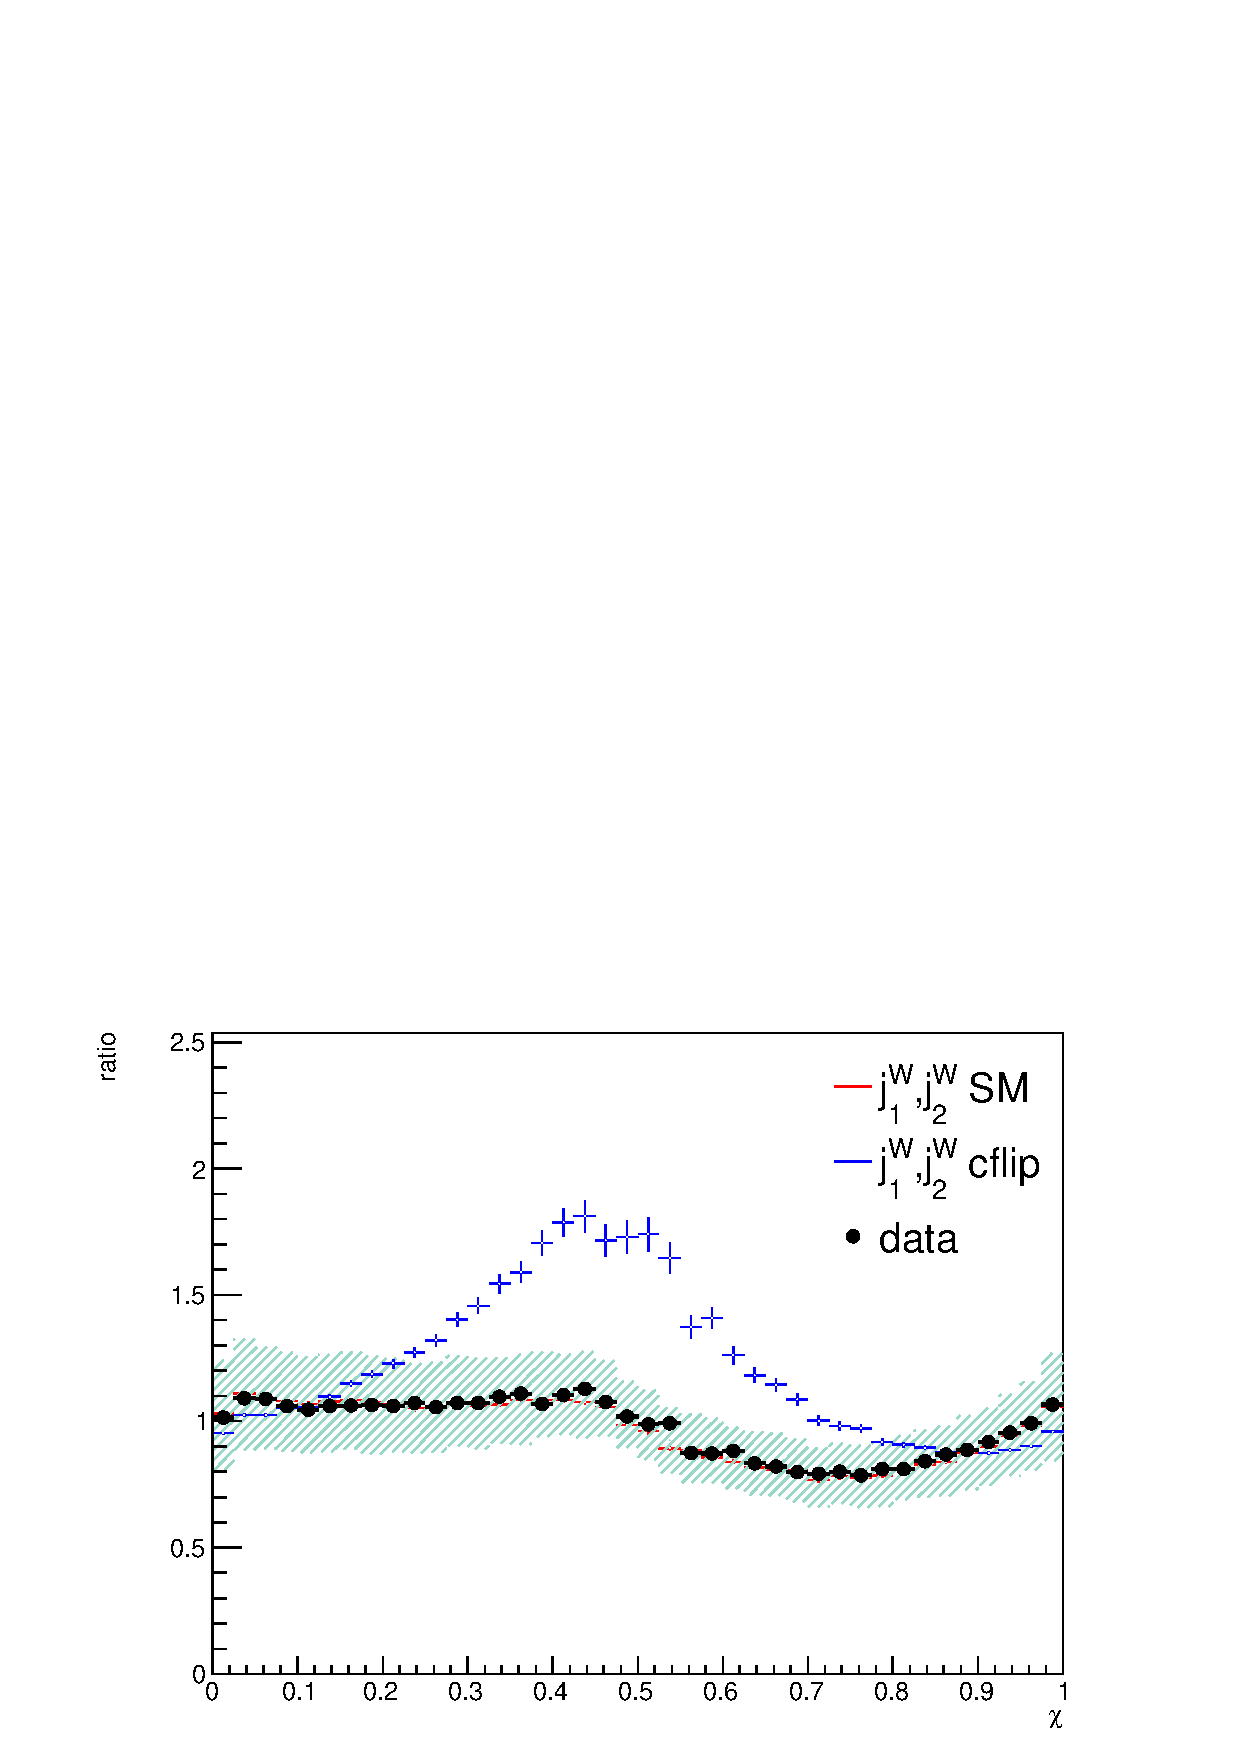
\includegraphics[width = 0.3\paperwidth]{\figrepository/ratiographs_merged_self/L_qcqf_N_allconst_reco.png}%
%%       \caption{$j_{c}^{W},j_{h}^{b}$}
%%     \end{subfigure}
%%     \begin{subfigure}[t]{0.3\paperwidth}
%%       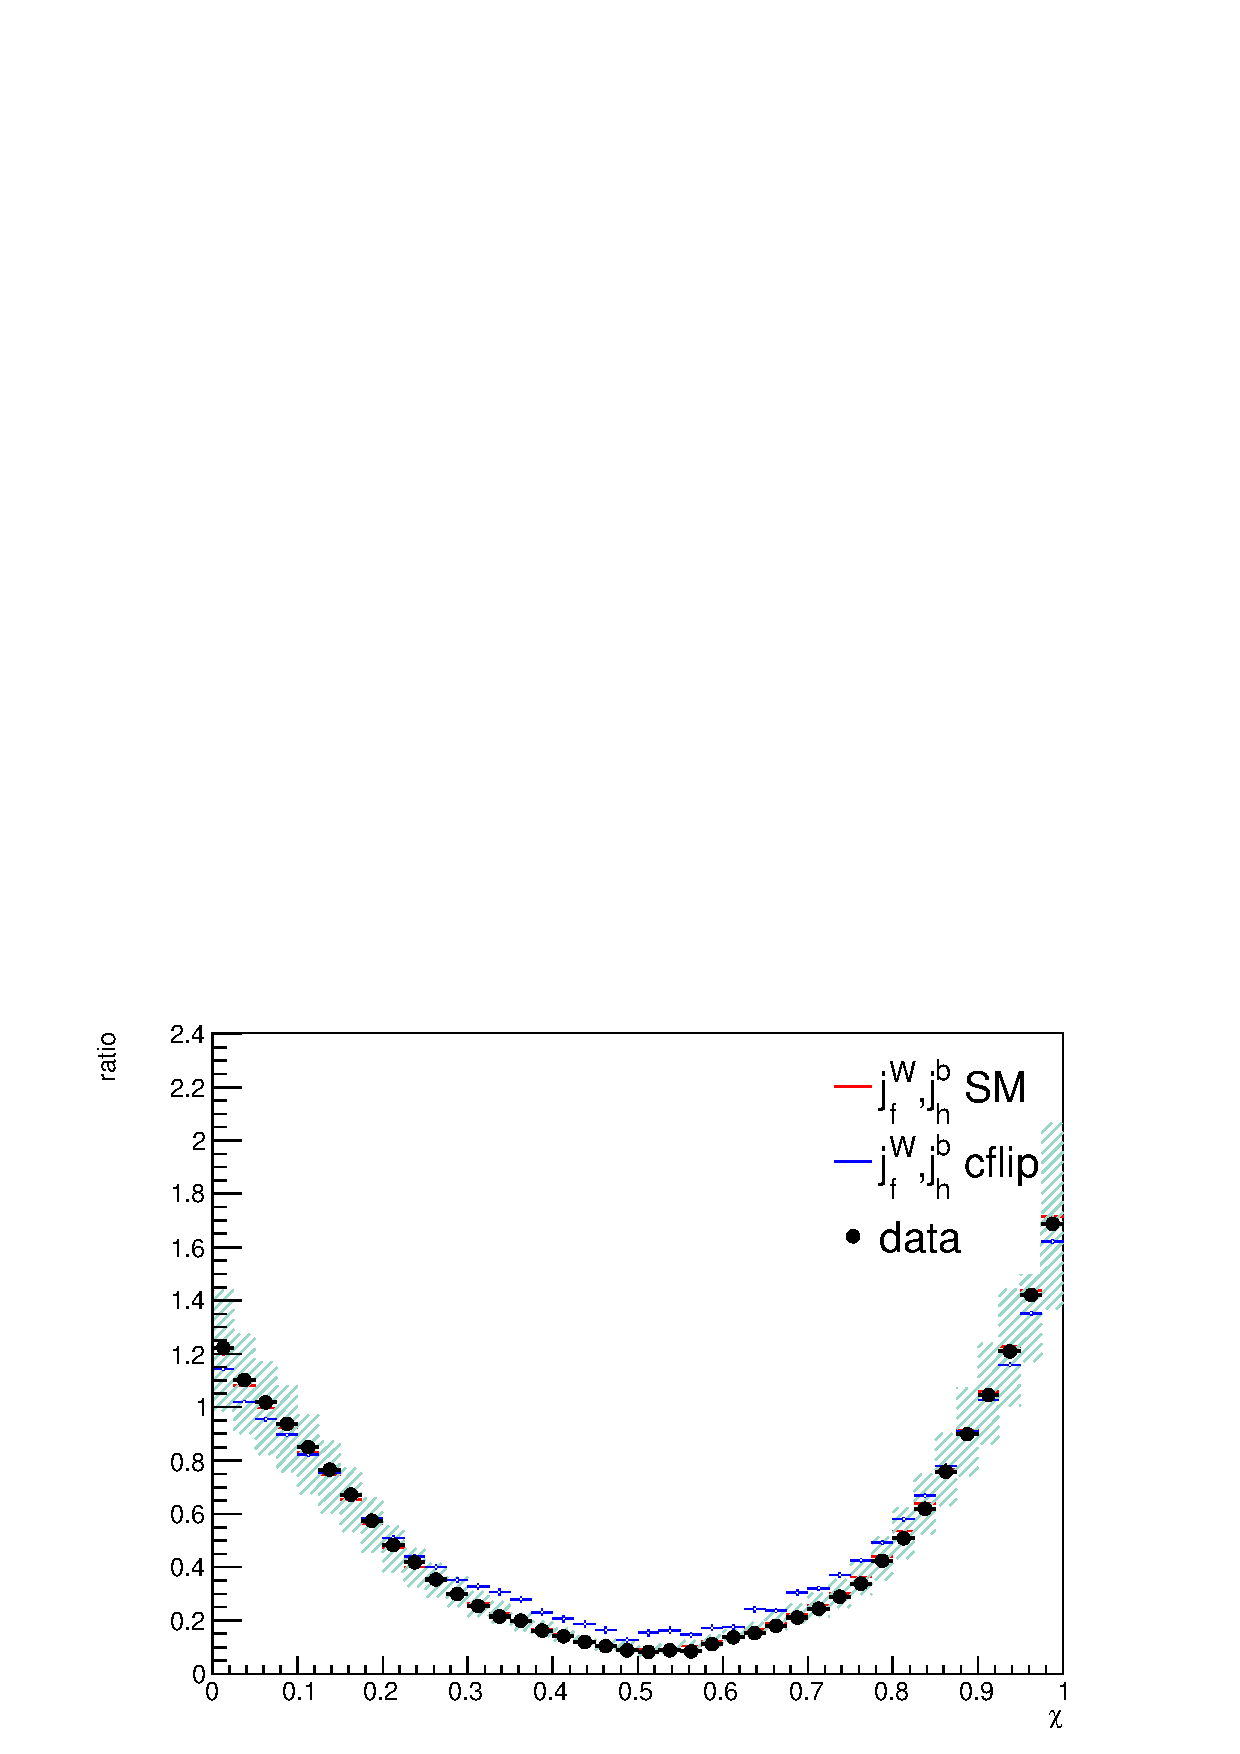
\includegraphics[width = 0.3\paperwidth]{\figrepository/ratiographs_merged_self/L_hbqf_N_allconst_reco.png}%
%%       \caption{$j_{h}^{b},j_{f}^{W}$}
%%     \end{subfigure}
%%     \begin{subfigure}[t]{0.3\paperwidth}
%%       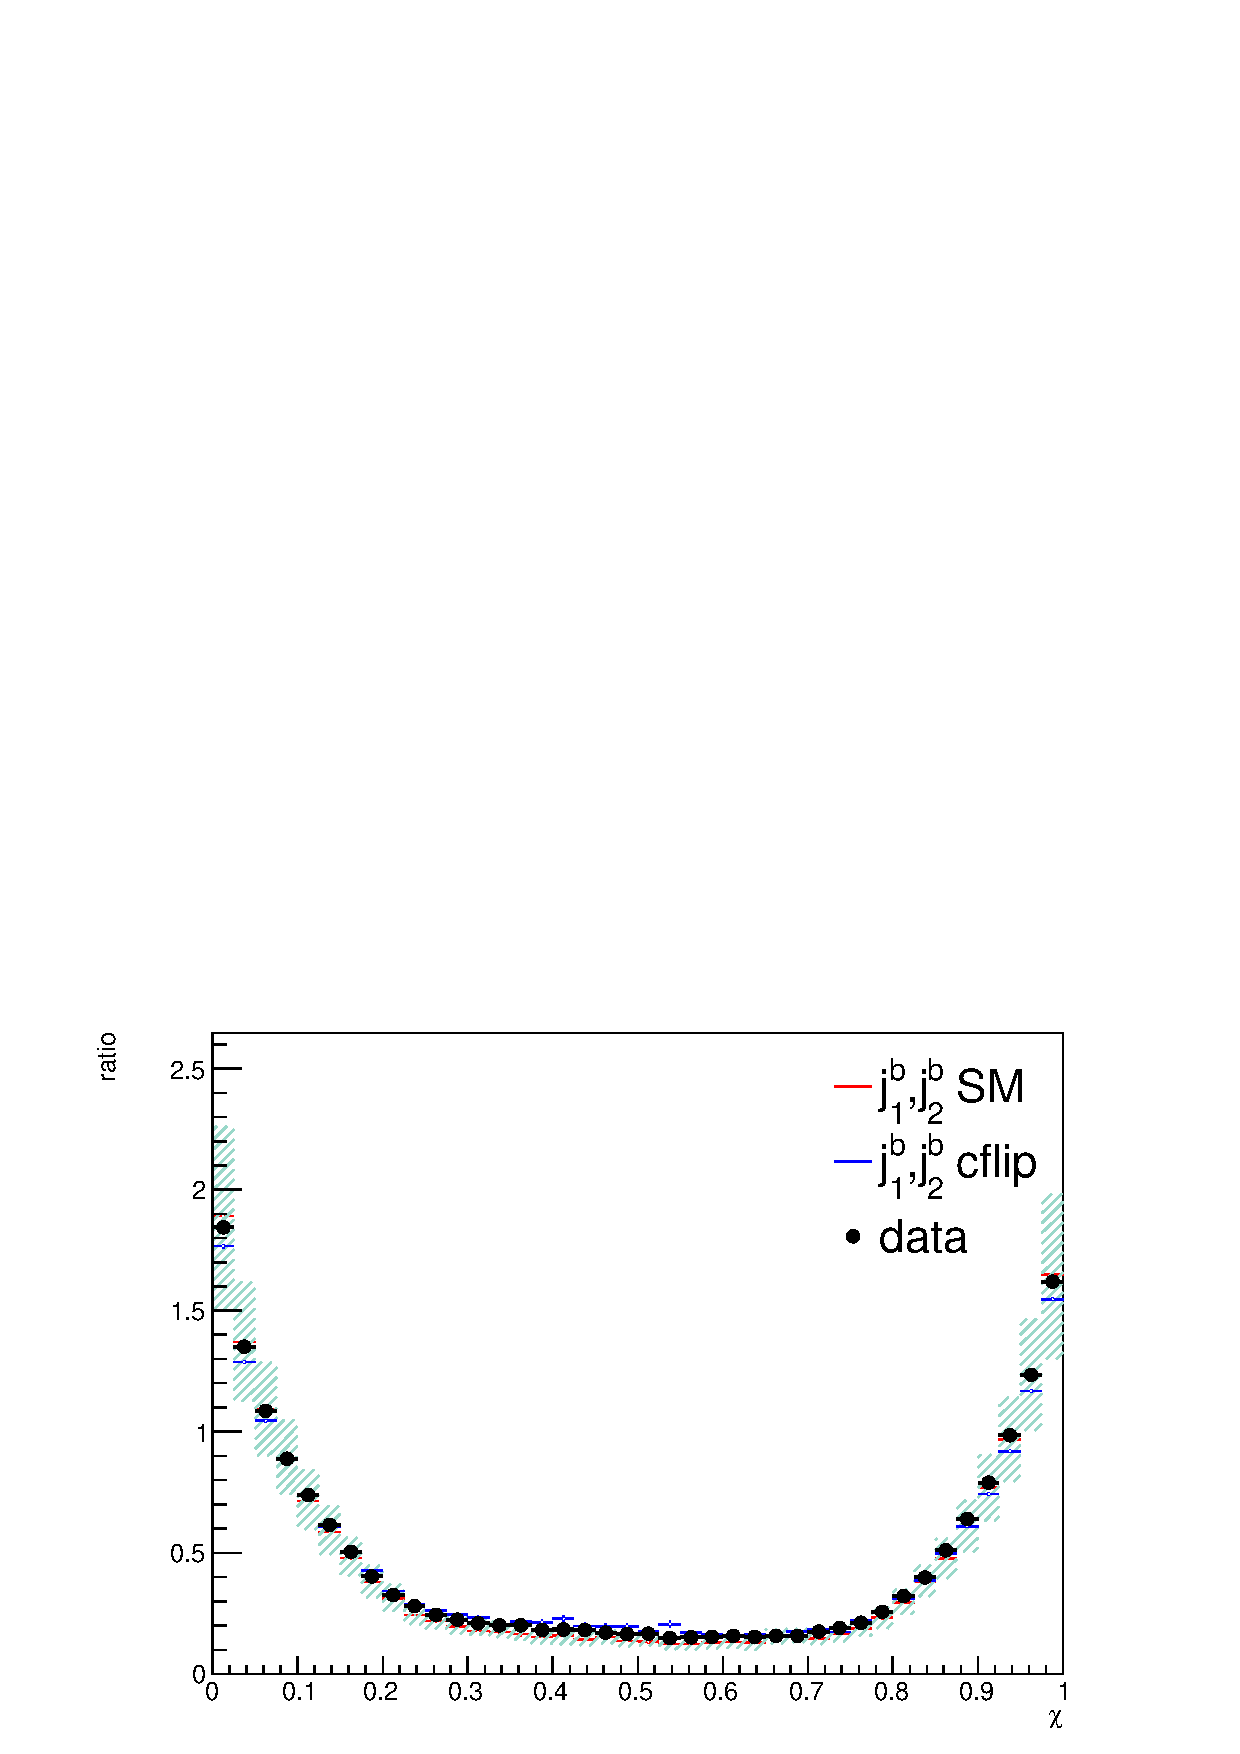
\includegraphics[width = 0.3\paperwidth]{\figrepository/ratiographs_merged_self/L_blb2l_N_allconst_reco.png}
%%       \caption{$j_{1}^{b},j_{2}^{b}$}
%%     \end{subfigure}
%%     \caption{}
%%   \end{figure}
%% \end{frame}

%% \begin{frame}{}
  
%%   \begin{figure}
%%       \includegraphics[width = 0.8\paperwidth]{\figrepository/ratiographs_merged_SM/L_hbqc_N_allconst_reco.png}%
%%   \end{figure}
%% \end{frame}

%% \begin{frame}{}
%%   %\tiny
%%   \input{tables/Rvalues_SM/R_L_reco_MC_N_SM.txt}
%% \end{frame}

%% \begin{frame}{}
%%   %\tiny
%%   \input{tables/Rvalues_SM/R_L_reco_data_N_SM.txt}
%% \end{frame}

%% \begin{frame}{}
%%   \input{tables/Rvalues_cflip/R_L_reco_MC_N_cflip.txt}
%% \end{frame}



%% \begin{frame}{The two hypothesis model}
%%   \begin{equation}
%%     q^{TEV}=-2\ln{\frac{L(H_{0})}{L(H_{alt})}}=-2\ln{\frac{L\left(\text{data}|p=0,\hat{\theta}_{0}\right)}{L\left(\text{data}|p=P,\hat{\theta}_{P}\right)}}
%%   \end{equation}

%%   \begin{equation}
%%     n=r\left(\left(1-x\right)f_{t\overline{t}} + xf_{t\overline{t}_{\text{cflip}}}\right) + b
%%     \label{eq:n}
%%   \end{equation}
%%   \begin{figure}[htp]
%%     \includegraphics[width=\textwidth]{\figrepository/npstatistic.pdf}
%%     \caption{}
%%     \label{fig:npstatistic}
%%   \end{figure}
  
%% \end{frame}

%% \begin{frame}
%%   \begin{figure}[htp]
%%     \includegraphics[width=0.8\textwidth]{\figrepository/hypox1.png}
%%     \caption{}
%%     \label{fig:TEVx1}
%%   \end{figure}
%%   $p_{0}=0.000$\\
%%   $p_{\text{alt}}=0.000$ 

%% \end{frame}

%% \begin{frame}
%%   \begin{figure}[htp]
%%     \includegraphics[width=0.8\textwidth]{\figrepository/likelihood.png}
%%     \caption{}
%%     \label{fig:TEVx1}
%%   \end{figure}

%% \end{frame}

%% \begin{frame}
%%   \begin{figure}[htp]
%%     \includegraphics[width=0.8\textwidth]{\figrepository/hypox0335.png}
%%     \caption{}
%%     \label{fig:TEVx0335}
%%   \end{figure}
%%   $p_{0}=0.000$\\
%%   $p_{\text{alt}}=0.249$ 
%%   \end{frame}


\end{document}
